% Document class
\documentclass{beamer}
\usecolortheme{default}
\usetheme{Madrid}
\usepackage{graphicx}
\usepackage{subfigure}

% Preamble
\title{Multivariate Time Series Modelling Of Ex-Pump Prices Of Petroleum Products In Ghana}
\subtitle{Chapter 4: Results and Discussions}
\author{Group 41}
\institute{Kwame Nkrumah University of Science and Technology}
\subject{Final Year Project}
\logo{
\includegraphics[width=20pt, height=20pt]{images/logo/logoKnust.png}}
\date{\today}

% Body
\begin{document}
	% Define variables
	\newcommand{\startDate}{January, 2007 }
	\newcommand{\finishDate}{June, 2015 }
	\newcommand{\numOfObservations}{204 }
	
	\newcommand{\highlight}{blue}
	\newcommand{\warning}{red}
	
	
	% Insert title here
	\begin{frame}
		\titlepage
	\end{frame}
	
	% Introduction
	\section{Introduction}
	\label{sec:introduction}
	\begin{frame}{Introduction}
		
		\begin{block}{Objective}
			The purpose of the study is to obtain a suitable model for the ex-pump prices of petroleum products in Ghana. 
		\end{block} \vspace{5pt}
		
		 To examines how changes in the prices of one product cause changes in the price of others in both the short and long terms. \par \vspace{5pt}
		
		Data spanning \startDate to \finishDate are obtained from the National Petroleum Authority of Ghana, covering four petroleum products; \textcolor{blue}{Gasoline, Gasoil, Kerosene, and Liquefied Petroleum Gas (LPG) }. 
	\end{frame}

	\begin{frame}{Chapter 4: Result And Discussion}
		This chapter analyses and discusses the results. It presents results of the association between the prices of the products considered, namely; \vspace{5pt}
		
		\begin{itemize}
			\item Gasoil
			\item Gasolin
			\item Kerosene 
			\item Liquefied Petroleum Gas (LPG)
		\end{itemize} \vspace{5pt}
		
		All associated tests and models are generated with R 
	\end{frame}
	
	
	% Descriptive Statistics
	\section{Descriptive Statistics}
	\label{sec:Descriptive}
	\begin{frame}{Descriptive Statistics}
		\begin{block}{}
			\vspace{4pt}
			In all, \numOfObservations observations are used (\startDate to \finishDate). \vspace{4pt}
		\end{block} \vspace{5pt}
		
		\begin{block}{}
		Training data of 144 observations (January 2007 to December 2012) for modelling \\ \vspace{5pt}
		
		Testing data of 60 data points (January 2013 to June 2015) for model validations.
		\end{block} \vspace{5pt}
	
		\begin{block}{}
			The descriptive statistics of the products are shown in Table \ref{table:description} on page \pageref{table:description}
		\end{block}
	\end{frame}

	\begin{frame}{Summary Statistics}
		\begin{table}[]
			\caption{ \ref{table:description} Summary Statistics}
			\begin{tabular}{lllll}
\hline
Statistics             & GASOIL  & GASOLINE & KEROSENE & LPG     \\ \hline
Mean                   & 122.445 & 123.570  & 82.989   & 94.766  \\
Maximum                & 175.480 & 177.090  & 120.420  & 136.190 \\
Minimum                & 11.600  & 49.170   & 6.470    & 58.500  \\
Standard Deviation     & 32.306  & 31.817   & 27.186   & 20.609  \\ 
Skewness               & -0.201  & 0.1307   & -1.988   & 0.413   \\
Kurtosis               & 3.374   & 2.123    & 6.293    & 2.292   \\
Number of Observations & 144     & 144      & 144      & 144     \\ \hline
			\end{tabular}
			\label{table:description}
		\end{table}
	\end{frame}

	\begin{frame}{Plot of Original Data}
		\begin{figure}
			\subfigure{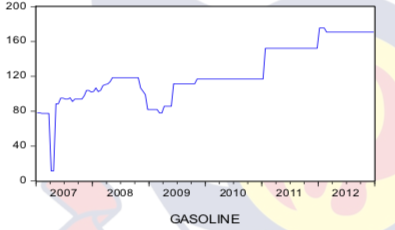
\includegraphics[height=0.3\textheight, width=0.4\textwidth]{images/plots/plot_original/plot_original_gasoline}}
			\subfigure{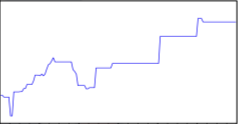
\includegraphics[height=0.3\textheight, width=0.4\textwidth]{images/plots/plot_original/plot_original_gasoil}}
			\subfigure{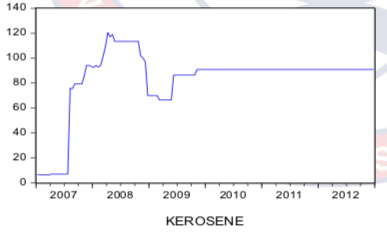
\includegraphics[height=0.3\textheight, width=0.4\textwidth]{images/plots/plot_original/plot_original_kerosene}}
			\subfigure{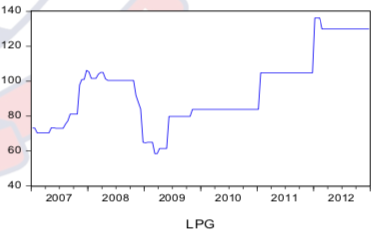
\includegraphics[height=0.3\textheight, width=0.4\textwidth]{images/plots/plot_original/plot_original_lpg}}
			
			
			\caption{ \ref{plot:original_data} Time Series Plot of the Original Series}
			\label{plot:original_data}
		\end{figure}
		
	\end{frame}
	
	% Trend and Stationarity Test
	\section{Trend And Stationarity Test}
	\begin{frame}{Trend Test}
		For trend test, We have chosen to apply
		
		\begin{block}{ Mann-Kendall Test}
			H0 : There is no monotonic trend in the dataset over time. \\
			H1 : There is a monotonic trend in the dataset over time. \vspace{5pt}
		\end{block}
		
		\begin{exampleblock}{Sen's Slope Test}
			H0 : There is no tonic trend in the dataset over time. \\
			H1 : There is a tonic trend in the dataset over time. \vspace{5pt}
		\end{exampleblock}
	\end{frame}

	\begin{frame}{Staionarity Test}
		We have numerous ways of testing for the presence of a unit root. 
		We have chosen to apply
		
		\begin{block}{Augmented Dickey-Fuller Test}
			H0 : The series is not stationary \\
			H1 : The series is stationary. \vspace{5pt}
		\end{block}
	
		\begin{exampleblock}{Phillips-Perron Unit Root Test}
			H0 : The series is not stationary \\
			H1 : The series is statrionary. \vspace{5pt}
		\end{exampleblock}
		
		\begin{alertblock}{KPSS Test for Level Stationarity}
			H0 : The series is stationary \\
			H1 : The series is not statrionary. \vspace{5pt}
		\end{alertblock}
	\end{frame}

	
	% Differencing
	
	
	% Estimation of VAR or VEC Models
	
	
	% LLS Criteria and Cointergration
	
	% Long and Short Term Equilibrium
	
	
	% Estimation of VEC Model
	
	
	% Model Validation
	
	
	% Forecast of Ex-Pump Prices of Products
	
	
	% Granger Gausality Test
	
	
	% Impurse Response Functions ( IRFs )
	
	% Summary of Results
	
	% Summary of Chapter
	
	
	
\end{document}